\section{Experiments and applications}
\label{sec:uses}

\subsection{Experimental setting}
\label{sec:uses:settings}

\paragraph{Implementation details.}
The simulations have been conducted in Python, including for the \palm algorithm.
Running times are measured on computer grid with 3.8GHz-CPUs (2.5GHz in Figure~\ref{fig:time_csr}).
Fast operators $\rmV$ based on sparse matrices $\rmS_q$ are implemented with \texttt{csr\_matrix} objects from the \texttt{scipy.linalg} package. 
While more efficient implementations may be beneficial for larger deployment, our implementation is sufficient as a proof of concept for assessing the performance of the proposed approach as illustrated by running times benchmarking in the Section~\ref{seq:sparse_factor_benchmarking} of supplementary material. \addLG{Je ne sais pas trop comment faire des références au supplementary material}
% In particular, the running times of fast operators of the form $\prod_{q\in\intint{\nfactors}}{\rmS_q}$ have been measured when applying to random vectors, for several sparsity levels: 
% as shown in Figure~\ref{fig:time_csr}, they are significantly faster than dense operators -- implemented as a \texttt{numpy.ndarray} matrix --, especially when the data size is larger than $10^3$.


% \begin{figure}[tbh]
% \centering
% 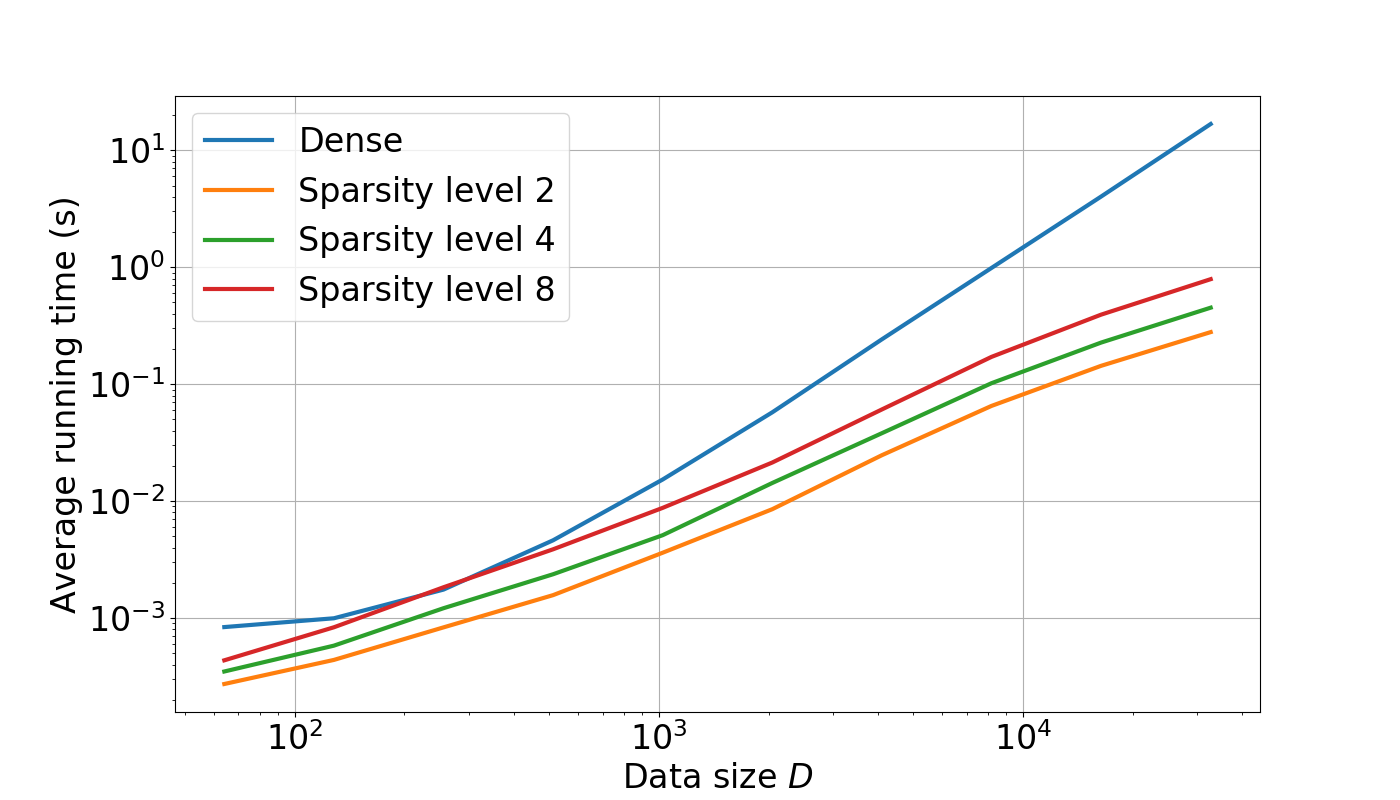
\includegraphics[width=.5\textwidth]{RunningTime4VaryingSparsity.png}
% \caption{Running times, averaged over 30 runs, when applying dense or fast $\datadim \times \datadim$ operators to a set of 100 random vectors. The number of factors in fast operators equals $\log_2\left (\datadim\right )$ and the sparsity level denotes the number of non-zero coefficients per row and per column in each factor.}
% \label{fig:time_csr}
% \end{figure}

%\begin{figure}[tbh]
%\centering
%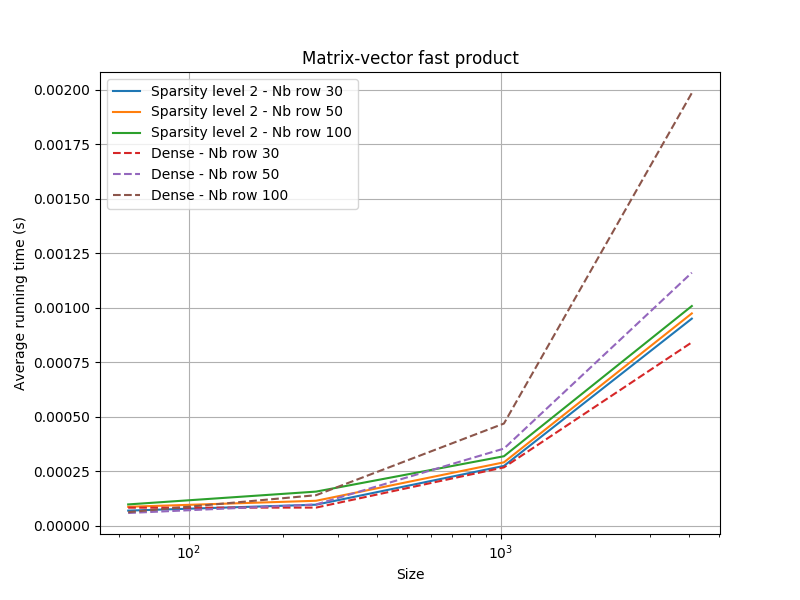
\includegraphics[width=.8\textwidth]{Run_time_sparsity_2.png}
%\caption{Running times, averaged over 30 runs, when applying dense or product of fast operators to a set of 100 random vectors. The number of factors in fast operators equals $\log_2\left (\#~row\right )$ and the sparsity level denotes the number of non-zero coefficients per row and per column in each factor.}
%\label{fig:time_csr_fixed_row_size}
%\end{figure}


\paragraph{Datasets.}
We present results on real-world and toy datasets summarized in supplementary material (Table \ref{table:data}) \addLG{Comment faire référence au supplementary material}. On the one hand, the real world datasets \texttt{MNIST}~\cite{lecun-mnisthandwrittendigit-2010} and \texttt{Fashion-Mnist}~\cite{Pedregosa2011Scikit} %and \texttt{Labeled Faces in the Wild}~\cite{Huang07e.:labeled} (\texttt{LFW}) 
are used to show --- quantitatively and qualitatively --- the good quality of the obtained centroids when using our method \qkmeans. On the other hand, we use the \texttt{blobs} synthetic dataset from \texttt{sklearn.dataset} to show the speed up offered by our method \qkmeans when the number of clusters and the dimensionality of the data are sufficiently large.
%The code of our method \qkmeans is available on request and will be available online soon. \addLG{je serais d'avis de ne pas dire ça mais soit de dire qu'il est déjà disponible, soit de ne rien dire. Sachant qu'on ne peut pas dire qu'il est déjà disponible en ligne avant le processus de reviewing}


% \begin{table*}[!h]
% \centering
% \begin{tabular}{|c|c|c|c|c|c|}
% \hline
% \textbf{Dataset} & \textbf{Data dim.} $\datadim$        & \textbf{\# classes} & \textbf{Training set size} $\nexamples$ & \textbf{Test set size} $\nexamples'$ \\ \hline
% MNIST                   & 784   & 10        & 60 000    & 10 000               \\ \hline
% Fashion-MNIST           & 784   & 10        & 60 000    & 10 000               \\ \hline
% % LFW                     & 1850  & 2529      & 8866      & N/A               \\ \hline
% Blobs (clusters std: 12)   & 2000  & 1000      & 29000      & 1000               \\ \hline
% \end{tabular}
% \caption{Datasets statistics}
% \label{table:data}
% \end{table*}


\paragraph{Algorithm settings.} 
The \qkmeans algorithm is used with $Q\eqdef\log_2\left (A\right )$ sparse factors, where  $A=\min\left (\nclusters, \datadim\right )$. 
All factors $\rmS_q$ are with shape $A \times A$ except, depending on the shape of $\rmA$, the leftmost one ($\nclusters\times A$) or the rightmost one ($A\times\datadim$). 
The sparsity constraint of each factor $\rmS_q$ is set in $\mathcal{E}_q$ and is governed by a global parameter denoted as \textit{sparsity level}, which indicates the desired number of non-zero coefficients in each row and in each column of $\rmS_q$. 
Since the projection onto this set of structured-sparsity constraints may be computationally expensive, this projection is relaxed in the implementation of \palm and only guarantees that the number of non-zero coefficients in each row and each column is at least the sparsity level, as in~\cite{LeMagoarou2016Flexible}.
The actual number of non-zero coefficients in the sparse factors is measured at the end of the optimization process and reported in the results.
The sparse factors are updated using the \palm rather than its hierarchical version, since we observed that this was a better choice in terms of computational cost, with satisfying approximation results (See Figure~\ref{fig:mnist:objfun}~and~\ref{fig:fmnist:objfun}).
Additional details about \palm are given in Appendix~\ref{sec:app:palm4msa}.
The stopping criterion of \kmeans and \qkmeans consists of a tolerance set to $10^{-6}$ on the relative variation of the objective function and a maximum number of iterations set to 10 for the \texttt{Blobs}dataset and to 20 for others. The same principle governs the stopping criterion of \palm with a tolerance set to $10^{-6}$ and a maximum number of iterations set to 300. Each experiment have been replicated using different seed values for random initialisation. Competing techniques share the same seed values, hence share the same initialisation of centroids.

%\subsection{Sparse factors multiplication}
%
%\subsubsection{Sparse factor object}

%\todo[inline]{Parler ici de la configuration de \qkmeans: $Q\eqdef\log_2\left (A\right )$, critère d'arrêt (nombre d'itération, tolérance), ordre des mises à jours, palm4msa plutôt que la version hiérarchique, taille des matrices $\rmS_q$, scaling coefficient, définition de 	$\mathcal{E}_q$.
%}

\subsection{Clustering}

\begin{figure*}[h]
\begin{subfigure}[b]{.49\textwidth}
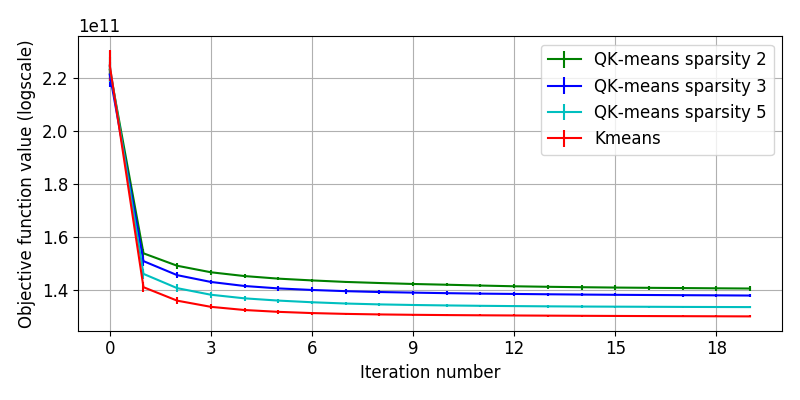
\includegraphics[width=\textwidth]{mnist30_objective.png}
\caption{MNIST, $\nclusters=30$: objective function.}
\label{fig:mnist:objfun}
\end{subfigure}
\begin{subfigure}[b]{.49\textwidth}
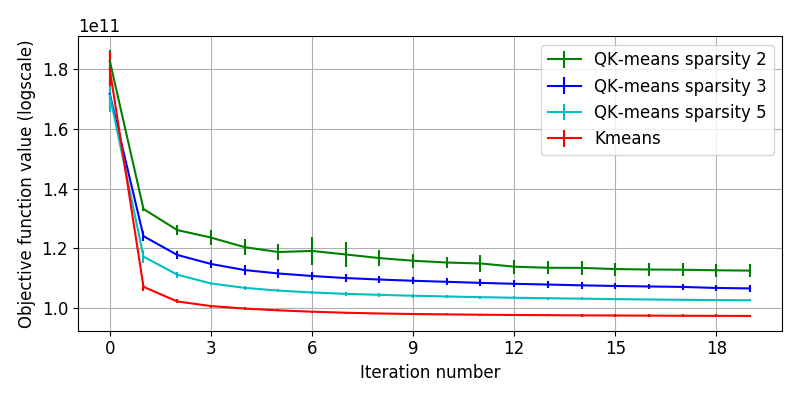
\includegraphics[width=\textwidth]{fashmnist30_objective.png}
\caption{Fashion-MNIST, $\nclusters=30$: objective function.}
\label{fig:fmnist:objfun}
\end{subfigure}
\begin{subfigure}[t]{.49\textwidth}
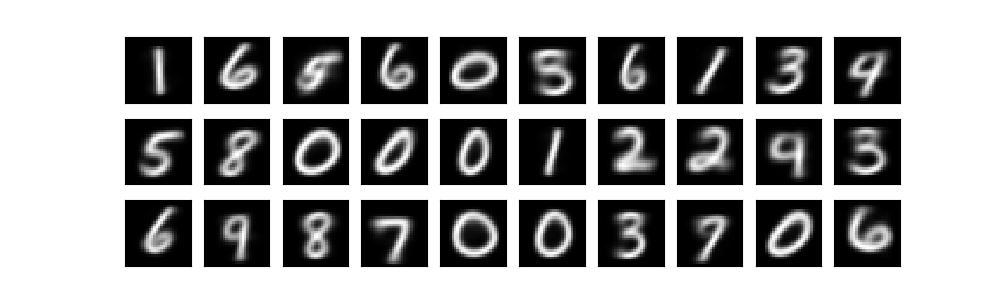
\includegraphics[width=\textwidth]{mnist30_kmeans_centroids.png}
\caption{\kmeans centroids.}
\label{fig:mnist:kmeans:centroids}
\end{subfigure}
\begin{subfigure}[t]{.49\textwidth}
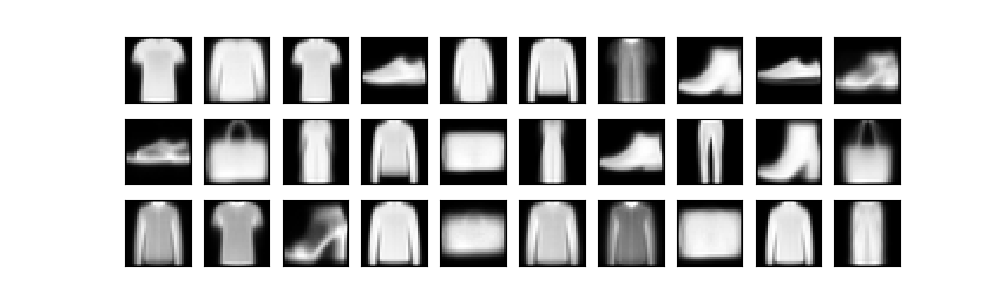
\includegraphics[width=\textwidth]{fashmnist30_kmeans_centroids.png}
\caption{\kmeans centroids.}
\label{fig:fmnist:kmeans:centroids}
\end{subfigure}
\begin{subfigure}[t]{.49\textwidth}
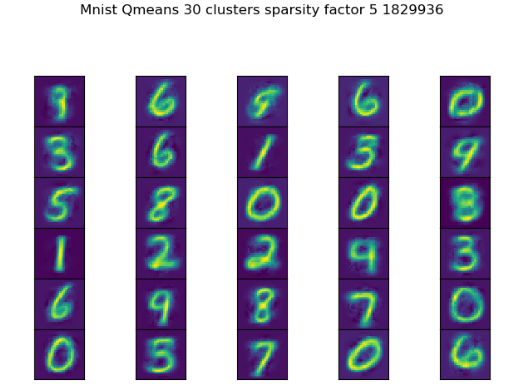
\includegraphics[width=\textwidth]{mnist30_qkmeans_centroids.png}
\caption{\qkmeans centroids.}
\label{fig:mnist:qkmeans:centroids}
\end{subfigure}
\begin{subfigure}[t]{.49\textwidth}
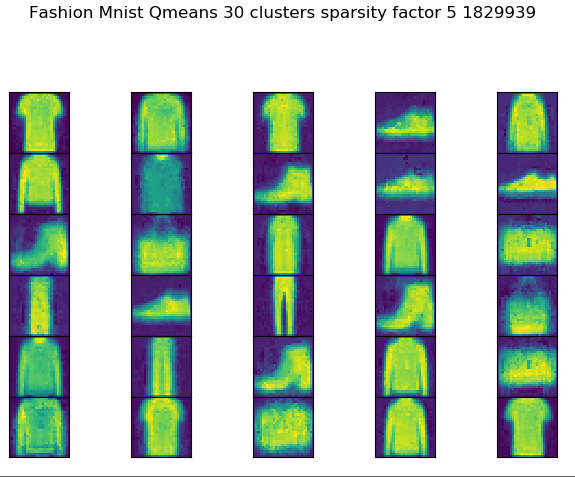
\includegraphics[width=\textwidth]{fashmnist30_qkmeans_centroids.png}
\caption{\qkmeans centroids.}
\label{fig:fmnist:qkmeans:centroids}
\end{subfigure}
% \begin{subfigure}[t]{.49\textwidth}
% 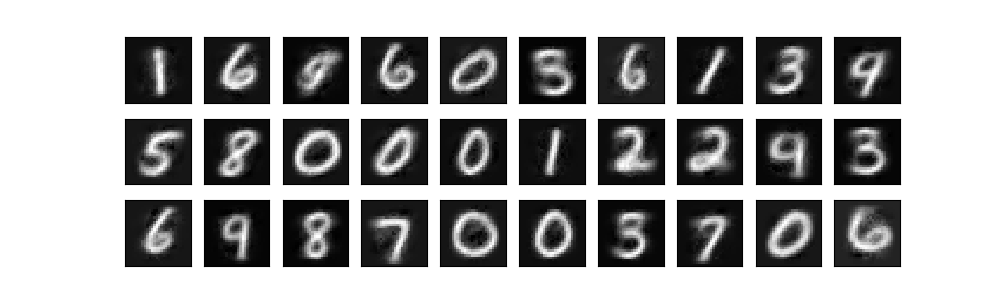
\includegraphics[width=\textwidth]{mnist30_hqkmeans_centroids.png}
% \caption{Hierarchical-\palm \qkmeans centroids.}
% \label{fig:mnist:hqkmeans:centroids}
% \end{subfigure}
% \begin{subfigure}[t]{.49\textwidth}
% 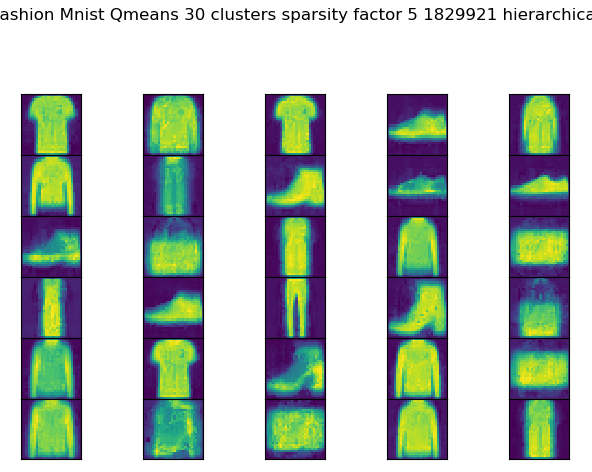
\includegraphics[width=\textwidth]{fashmnist30_hqkmeans_centroids.png}
% \caption{Hierarchical-\palm \qkmeans centroids.}
% \label{fig:fmnist:hqkmeans:centroids}
% \end{subfigure}
\caption{Clustering results on MNIST (left) and Fashion-MNIST (right) for $\nclusters=30$ clusters.}
\label{fig:clustering:realdata}
\end{figure*}

\paragraph{Approximation quality.} One important question is the ability of the fast-structure model to fit arbitrary data.
Indeed, no theoretical result about the expressivity of such models is currently available.
In order to assess this approximation quality, the MNIST and Fashion-MNIST data have been clustered into $\nclusters=30$ clusters by \kmeans, \qkmeans and a variant of \qkmeans using the hierarchical version of \palm, with several sparsity levels.
Results are reported in Figure~\ref{fig:clustering:realdata}.
In Figures~\ref{fig:mnist:objfun} and~\ref{fig:fmnist:objfun}, one can observe that the objective function of \qkmeans is decreasing in a similar way as \kmeans over iterations.
In particular, the use of the fast-structure model does not seem to increase the number of iteration necessary before convergence.
At the end of the iterations, the value of objective function for \qkmeans is slightly above that of \kmeans.
As expected, the sparser the model, the more degradation in the objective function.
However, even very sparse models do not degrade the results significantly. These Figures also demonstrate the convergence property of the \qkmeans algorithm when using the standard, proved convergent, \textit{Palm4MSA} algorithm: in this case, the objective function is always non-increasing whereas the \qkmeans version with \textit{Hiearchical Palm4MSA}, not guaranteed to converge, suffers a small bump in its objective function (see Figure~\ref{fig:fmnist:objfun} iteration~6).
The approximation quality can be assessed visually, in a more subjective and interpretable way, in Figures~\ref{fig:mnist:kmeans:centroids} to~\ref{fig:fmnist:hqkmeans:centroids} where the obtained centroids are displayed as images.
Although some degradation may be observed in some images, one can note that each image obtained with \qkmeans clearly represents a single visual item without noticeable interference with other items.

\paragraph{Clustering assignation times.}
Higher dimensions are required to assess the computational benefits of the proposed approach, as shown here.
The assignation times of the clustering procedure were measured on the \texttt{Blobs} dataset.
The centroid matrices are with shape $\nclusters \times \datadim$ with $\datadim=2000$  and $\nclusters\in\left \lbrace 128, 256, 512\right \rbrace$.
Results reported in Figure~\ref{fig:clustering:blobs:assignation_time} show that in this setting and with the current implementation, the computational advantage of \qkmeans is observed in high dimension, for $\nclusters=256$ and $\nclusters=512$ clusters. It is worth noticing that when $K$ increases, the running times are not affected that much for \qkmeans while it significantly grows for \kmeans. These trends are directly related to the number of model parameters that are reported in the figure.


%\todo[inline]{Montrer ensuite les temps d'assignation en mode batch 5000 sur blobs, cf. Figure~\ref{fig:clustering:blobs:assignation_time}. Objectif: montrer qu'à partir d'une certaine dimension, \qkmeans est plus rapide.}
%on-line\footnote{Anonymous URL.}.

\begin{figure}[tbh]
\centering
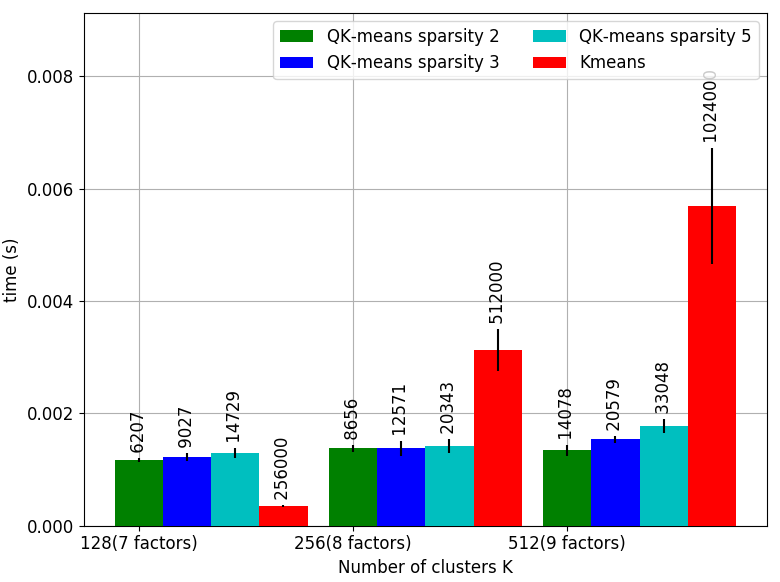
\includegraphics[width=.45\textwidth]{blobs_assignation_time.png}
\caption{Clustering Blobs data: running times of the assignation step, averaged over 5 runs. The vertical black lines are the standard deviation w.r.t. the runs and the average number of parameters actually learned  in the models are reported above those lines.\addVE{to be completed}.}
\label{fig:clustering:blobs:assignation_time}
\end{figure}

\subsection{Nearest-neighbor search in a large dataset}
The Nearest-neighbor search is a fundamental task that suffers from computational limitations when the dataset is large.
Fast strategies have been proposed, e.g., using kd trees or ball trees.
One may also use a clustering strategy to perform an approximate nearest-neighbor search: the query is first compared to $\nclusters$ centroids computed beforehand by clustering the whole dataset, and the nearest neighbor search is then performed among a lower number of data points, within the related cluster.
We compare this strategy using \kmeans and \qkmeans against the \texttt{scikit-learn} implementation~\cite{Pedregosa2011Scikit} of the nearest-neighbor search (brute force search, kd tree, ball tree).
Inference time results on the \texttt{Blobs} dataset are reported in Figure~\ref{fig:nn:blobs} and accuracy results are displayed in Table~\ref{table:results_blobs}. 
% As shown in Figure~\ref{fig:nn:blobs:accuracy}, the accuracy of the approximate nearest neighbor search is above $0.99$ \todo{Accuracy $>0.99$ to be checked} for all the tested variants of \qkmeans, which is an solid evidence about the reliability of the approach.
The running times reported in Figure~\ref{fig:nn:blobs} show a dramatic advantage of using a clustering-based approximate search 
%\todo{to be completed by reporting the actual acceleration ratio obtained by \qkmeans over the three sklearn options.} 
and this advantage is even stronger with the clustering obtained by our \qkmeans method. This speed-up comes at a cost though, we can see a drop in classification performance in Table~\ref{table:results_blobs}. 

\begin{figure}[tbh]
\centering
%\begin{subfigure}[b]{.49\textwidth}
%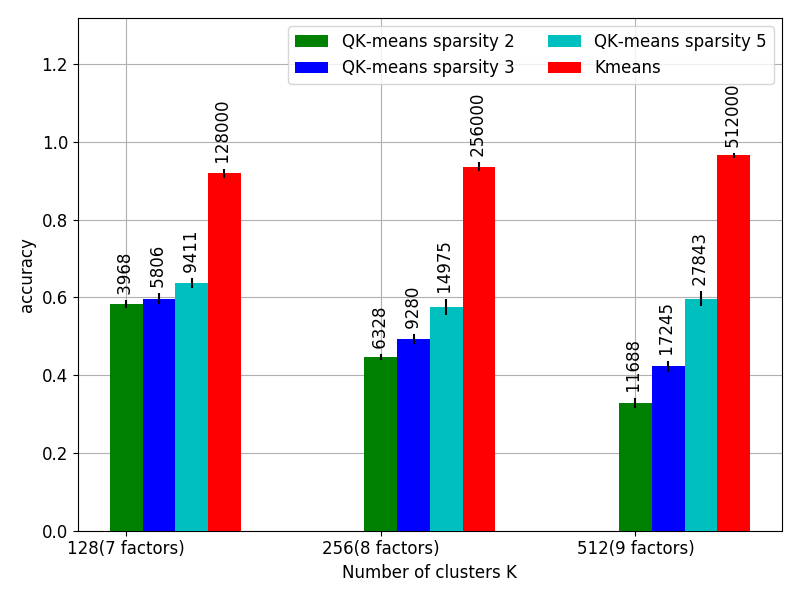
\includegraphics[width=\textwidth]{blobs_1nn_accuracy.png}
%\caption{Accuracy.}
%\label{fig:nn:blobs:accuracy}
%\end{subfigure}
%\begin{subfigure}[b]{.49\textwidth}
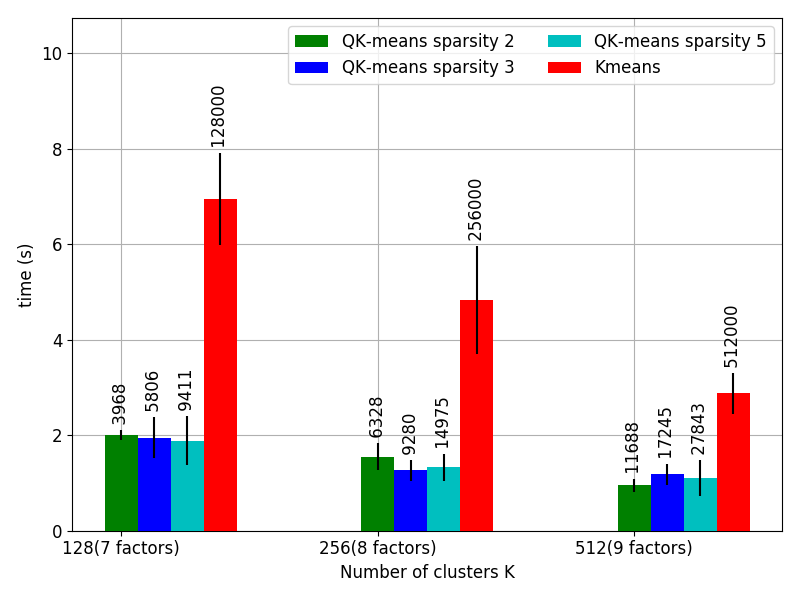
\includegraphics[width=.45\textwidth]{blobs_1nn_inference_time.png}
%\caption{Running times.}
\label{fig:nn:blobs:times}
%\end{subfigure}

\caption{Running time of nearest neighbor search on blobs data. Results are averaged over 5 runs (vertical lines: standard deviation) and the average number of parameters actually learned is reported above each bar. The results for the Brute Force Search, KD Tree and Ball Tree are not displayed because they were longer than 10 times the K-means search version.}
\label{fig:nn:blobs}
\end{figure}


% \begin{table*}[!htb]
% \caption{Results on the classification task. Results are averaged over 5 runs. ``N/A'' denotes experiments that did not finish. For the \qkmeans results, only those obtained with sparsity level = 5 are displayed.}
% \centering
% \begin{adjustbox}{max width=0.8\textwidth}
% \begin{minipage}{.5\linewidth}
% % \centering
% \begin{tabular}{@{}lc}
% \toprule
%                                     & \thead{Accuracy \\ \texttt{Blobs}} \\ \midrule
% 1NN Brute force search              & N/A   \\
% 1NN KD Tree                         & N/A   \\
% 1NN Ball Tree                       & N/A   \\ \midrule \midrule
% 1NN K-means 128 Clusters            & 0.96      \\
% 1NN K-means 256 Clusters            & 0.97      \\
% 1NN K-means 512 Clusters            & 0.99      \\ \midrule
% 1NN QK-means 128 Clusters           & 0.74     \\
% 1NN QK-means 256 Clusters           & 0.66      \\
% 1NN QK-means 512 Clusters           & 0.66      \\ \midrule \midrule
% Nyström K-means + SVM 128 Clusters  & 0.98      \\
% Nyström K-means + SVM 256 Clusters  & 1.0      \\
% Nyström K-means + SVM 512 Clusters  & 1.0      \\ \midrule
% Nyström QK-means + SVM 128 Clusters & 0.95      \\
% Nyström QK-means + SVM 256 Clusters & 1.0      \\
% Nyström QK-means + SVM 512 Clusters & 1.0      \\ \bottomrule
% \end{tabular}
% \caption{\texttt{Blobs} dataset}
% \end{minipage}%
% \begin{minipage}{.5\linewidth}
% % \centering
% \begin{tabular}{@{}lcc}
% \toprule
%                                     & \thead{Accuracy \\ \texttt{Fashion-MNIST}} & \thead{Accuracy \\ \texttt{MNIST}} \\ \midrule
% 1NN Brute force search              &  0.85   &  0.97 \\
% 1NN KD Tree                         & 0.85  &  0.97  \\
% 1NN Ball Tree                       & 0.85  &  0.97  \\ \midrule \midrule
% 1NN K-means 10 Clusters            & 0.84  &  0.96  \\
% 1NN K-means 16 Clusters            & 0.84  &  0.96  \\
% 1NN K-means 30 Clusters            & 0.84  &  0.96  \\ \midrule
% 1NN QK-means 10 Clusters           & 0.84  &  0.96  \\
% 1NN QK-means 16 Clusters           & 0.84  &  0.96  \\
% 1NN QK-means 30 Clusters           & 0.84  &  0.96  \\ \midrule \midrule
% Nyström K-means + SVM 10 Clusters  &  0.71  & 0.74  \\
% Nyström K-means + SVM 16 Clusters  &  0.75  & 0.83  \\
% Nyström K-means + SVM 30 Clusters  &  0.78  & 0.88  \\ \midrule
% Nyström QK-means + SVM 10 Clusters &  0.71  & 0.74  \\
% Nyström QK-means + SVM 16 Clusters &  0.74  & 0.82  \\
% Nyström QK-means + SVM 30 Clusters &  0.77  & 0.88  \\ \bottomrule
% \end{tabular}
% \caption{\texttt{MNIST} and \texttt{Fashion-MNIST} datasets}
% \end{minipage}
% \end{adjustbox}
% \end{table*}

\begin{table*}[!htb]
\begin{adjustbox}{center, max width=0.9\textwidth}

\begin{subtable}{.5\textwidth}
% \centering
\begin{tabular}{@{}lc}
\toprule
                                    & \thead{Accuracy \\ \texttt{Blobs}} \\ \midrule
1NN Brute force search              & N/A   \\
1NN KD Tree                         & N/A   \\
1NN Ball Tree                       & N/A   \\ \midrule \midrule
1NN K-means 128 Clusters            & 0.96      \\
1NN K-means 256 Clusters            & 0.97      \\
1NN K-means 512 Clusters            & 0.99      \\ \midrule
1NN QK-means 128 Clusters           & 0.74     \\
1NN QK-means 256 Clusters           & 0.66      \\
1NN QK-means 512 Clusters           & 0.66      \\ \midrule \midrule
Nyström K-means + SVM 128 Clusters  & 0.98      \\
Nyström K-means + SVM 256 Clusters  & 1.0      \\
Nyström K-means + SVM 512 Clusters  & 1.0      \\ \midrule
Nyström QK-means + SVM 128 Clusters & 0.95      \\
Nyström QK-means + SVM 256 Clusters & 1.0      \\
Nyström QK-means + SVM 512 Clusters & 1.0      \\ \bottomrule
\end{tabular}
\caption{\texttt{Blobs} dataset}

\end{subtable}%
\begin{subtable}{.5\textwidth}
% \centering
\begin{tabular}{@{}lcc}
\toprule
                                    & \thead{Accuracy \\ \texttt{Fashion-MNIST}} & \thead{Accuracy \\ \texttt{MNIST}} \\ \midrule
1NN Brute force search              &  0.85   &  0.97 \\
1NN KD Tree                         & 0.85  &  0.97  \\
1NN Ball Tree                       & 0.85  &  0.97  \\ \midrule \midrule
1NN K-means 10 Clusters            & 0.84  &  0.96  \\
1NN K-means 16 Clusters            & 0.84  &  0.96  \\
1NN K-means 30 Clusters            & 0.84  &  0.96  \\ \midrule
1NN QK-means 10 Clusters           & 0.84  &  0.96  \\
1NN QK-means 16 Clusters           & 0.84  &  0.96  \\
1NN QK-means 30 Clusters           & 0.84  &  0.96  \\ \midrule \midrule
Nyström K-means + SVM 10 Clusters  &  0.71  & 0.74  \\
Nyström K-means + SVM 16 Clusters  &  0.75  & 0.83  \\
Nyström K-means + SVM 30 Clusters  &  0.78  & 0.88  \\ \midrule
Nyström QK-means + SVM 10 Clusters &  0.71  & 0.74  \\
Nyström QK-means + SVM 16 Clusters &  0.74  & 0.82  \\
Nyström QK-means + SVM 30 Clusters &  0.77  & 0.88  \\ \bottomrule
\end{tabular}
\caption{\texttt{MNIST} and \texttt{Fashion-MNIST} datasets}
\label{table:results_mnist_fmnist}
\end{subtable}
\end{adjustbox}
\caption{Results on the classification task. Results are averaged over 5 runs. ``N/A'' denotes experiments that did not finish. For the \qkmeans results, only those obtained with sparsity level = 5 are displayed.}
\end{table*}


% \begin{table*}[]
% 
% \centering
% \begin{tabular}{@{}l|P{2.5cm}}
% \toprule
%                                     & Accuracy \texttt{Blobs} \\ \midrule
% 1NN Brute force search              & N/A   \\
% 1NN KD Tree                         & N/A   \\
% 1NN Ball Tree                       & N/A   \\ \midrule \midrule
% 1NN K-means 128 Clusters            & 0.96      \\
% 1NN K-means 256 Clusters            & 0.97      \\
% 1NN K-means 512 Clusters            & 0.99      \\ \midrule
% 1NN QK-means 128 Clusters           & 0.74     \\
% 1NN QK-means 256 Clusters           & 0.66      \\
% 1NN QK-means 512 Clusters           & 0.66      \\ \midrule \midrule
% Nyström K-means + SVM 128 Clusters  & 0.98      \\
% Nyström K-means + SVM 256 Clusters  & 1.0      \\
% Nyström K-means + SVM 512 Clusters  & 1.0      \\ \midrule
% Nyström QK-means + SVM 128 Clusters & 0.95      \\
% Nyström QK-means + SVM 256 Clusters & 1.0      \\
% Nyström QK-means + SVM 512 Clusters & 1.0      \\ \bottomrule
% \end{tabular}
% 
% %\caption{}
% \label{table:results_blobs}

% \end{table*}

% \begin{table*}[]

% \centering

% \begin{tabular}{@{}l|P{2.5cm}|P{2.5cm}}
% \toprule
%                                     & Accuracy \texttt{Fashion-MNIST} & Accuracy \texttt{MNIST} \\ \midrule
% 1NN Brute force search              &  0.85   &  0.97 \\
% 1NN KD Tree                         & 0.85  &  0.97  \\
% 1NN Ball Tree                       & 0.85  &  0.97  \\ \midrule \midrule
% 1NN K-means 10 Clusters            & 0.84  &  0.96  \\
% 1NN K-means 16 Clusters            & 0.84  &  0.96  \\
% 1NN K-means 30 Clusters            & 0.84  &  0.96  \\ \midrule
% 1NN QK-means 10 Clusters           & 0.84  &  0.96  \\
% 1NN QK-means 16 Clusters           & 0.84  &  0.96  \\
% 1NN QK-means 30 Clusters           & 0.84  &  0.96  \\ \midrule \midrule
% Nyström K-means + SVM 10 Clusters  &  0.71  & 0.74  \\
% Nyström K-means + SVM 16 Clusters  &  0.75  & 0.83  \\
% Nyström K-means + SVM 30 Clusters  &  0.78  & 0.88  \\ \midrule
% Nyström QK-means + SVM 10 Clusters &  0.71  & 0.74  \\
% Nyström QK-means + SVM 16 Clusters &  0.74  & 0.82  \\
% Nyström QK-means + SVM 30 Clusters &  0.77  & 0.88  \\ \bottomrule
% \end{tabular}

% \caption{}
% \label{table:results_mnist_fmnist}
% 
% \end{table*}

\subsection{Nyström approximation}

In this sub-section, we show how we can take advantage of the fast-operator obtained as output of our \qkmeans algorithm in order to speed-up the computation in the Nyström approximation. 
We start by giving background knowledge on the Nyström approximation then we present some recent work aiming at accelerating it using well know fast-transform method. 
We finally stem on this work to present a novel approach based on our \qkmeans algorithm.

\subsubsection{Background on the Nyström approximation}

Standard kernel machines are often impossible to use in large-scale applications because of their high computational cost associated with the kernel matrix $\rmK$ which has $O(n^2)$ storage and $O(n^2d)$ computational complexity: $\forall i,j \in\intint{\nexamples}, \rmK_{i,j} = k(\rvx_i, \rvx_j)$. A well-known strategy to overcome this problem is to use the Nyström method which computes a low-rank approximation of the kernel matrix on the basis of some pre-selected landmark points. 

Given $K \ll n$ landmark points $\{\rmU_i\}_{i=1}^{K}$, the Nyström method gives the following approximation of the full kernel matrix:
%
\begin{equation}
 \label{eq:nystrom}
 \rmK \approx \tilde\rmK = \rmC\rmW^\dagger\rmC^T,
\end{equation}
%
with $\rmW \in \R^{K \times K}$ containing all the kernel values between landmarks: $\forall i,j \in [\![K]\!]~ \rmW_{i,j} = k(\rmU_i, \rmU_j)$; $\rmW^\dagger$ being the pseudo-inverse of $\rmW$ and $\rmC \in \R^{n \times K}$ containing the kernel values between landmark points and all data points: $\forall i \in [\![n]\!], \forall j \in [\![K]\!]~ \rmC_{i, j} = k(\rmX_i, \rmU_j)$.

\subsubsection{Efficient Nyström approximation}

A substantial amount of research has been conducted toward landmark point selection methods for improved approximation accuracy \cite{kumar2012sampling} \cite{musco2017recursive}, but much less has been done to improve computation speed. In \cite{si2016computationally}, the authors propose an algorithm to learn the matrix of landmark points with some structure constraint, so that its utilisation is fast, taking advantage of fast-transforms. This results in an efficient Nyström approximation that is faster to use both in the training and testing phases of some ulterior machine learning application.

Remarking that the main computation cost of the Nyström approximation comes from the computation of the kernel function between the train/test samples and the landmark points, \cite{si2016computationally} aim at accelerating this step. In particular, they focus on a family of kernel functions that has the following form:
%
\begin{equation}
 k(\rvx_i, \rvx_j) = f(\rvx_i) f(\rvx_j) g(\rvx_i^T\rvx_j),
\end{equation}
%
where $f: \R^d \rightarrow \R$ and $g: \R \rightarrow \R$. They show that this family of functions contains some widely used kernels such as the Gaussian and the polynomial kernel. Given a set of $K$ landmark points $\rmU \in \R^{K \times d}$ and a sample $\rvx$, the computational time for computing the kernel between $\rvx$ and each row of $\rmU$ (necessary for the Nyström approximation) is bottlenecked by the computation of the product $\rmU\rvx$. They hence propose to write the $\rmU$ matrix as the concatenation of structured $s = K / d$ product of matrices:
%
\begin{equation}
 \rmU = \left[ \rmV_1 \rmH^T, \cdots, \rmV_s\rmH^T  \right]^T,
\end{equation}
%
where the $\rmH$ is a $d \times d$ matrix associated with a fast transform such as the \textit{Haar} or \textit{Hadamard} matrix, and the $\rmV_i$s are some $d \times d$ diagonal matrices to be either chosen with a standard landmark selection method or learned using an algorithm they provide.

Depending on the $\rmH$ matrix chosen, it is possible to improve the time complexity for the computation of $\rmU\rvx$ from $O(Kd)$ to $O(K \log{d})$ (\textit{Fast Hadamard transform}) or $O(K)$ (\textit{Fast Haar Transform}).

\subsubsection{\qkmeans in Nyström}

We propose to use our \qkmeans algorithm in order to learn directly the $\rmU$ matrix in the Nyström approximation so that the matrix-vector multiplication $\rmU \rvx$ is cheap to compute, but the structure of $\rmU$ is not constrained by some pre-defined transform matrix. We propose to take the objective $\rmU$ matrix as the \kmeans matrix of $\rmX$ since it has been shown to achieve good reconstruction accuracy in the Nyström method \cite{kumar2012sampling}.

As shown in the next sub-section, our algorithm allow to obtain an efficient Nyström approximation, while not reducing too much the quality of the \kmeans landmark points which are encoded as a factorization of sparse matrix. 

\subsubsection{Results}

The Figure~\ref{fig:nystrom} summarizes the results achieved in the Nyström approximation setting. 

The Figures on the right display the average time for computing one line of the approximated matrix in Equation~\ref{eq:nystrom}. In Figure~\ref{fig:blobs:nystrom_time}, we clearly see the speed-up offered using the \qkmeans method on the \texttt{Blobs} dataset. On the \texttt{Mnist} and \texttt{Fashion-MNIST} dataset (Figure~\ref{fig:mnist:nystrom_time}~and~\ref{fig:fashmnist:nystrom_time}), this speed-up is sensible but not as clear because the standard deviation is much larger. 

The Figures on the left show the approximation error of the Nyström approximation based on different sampling schemes w.r.t. the real kernel matrix. This error is computed by the Froebenius norm of the difference between the matrices and then normalized:

\begin{equation}
 error = \frac{||\rmK - \tilde\rmK||_F}{||\rmK||_F}
\end{equation}

. The \qkmeans approach gives better reconstruction error than the Nyström method based on uniform sampling although they are slightly worse than the one obtained with the \kmeans centroids. We see that that the difference in approximation error between \kmeans and \qkmeans is almost negligeable when compared to the approximation error obtained with the uniform sampling scheme.

From a more practical point of view, we show in Table~\ref{table:results_blobs} and Table~\ref{table:results_mnist_fmnist} that the Nyström approximation based on \qkmeans can then be used in a linear SVM and achieve as good performance as the one based on the \kmeans approach.


\begin{figure*}
\begin{subfigure}[b]{.49\textwidth}
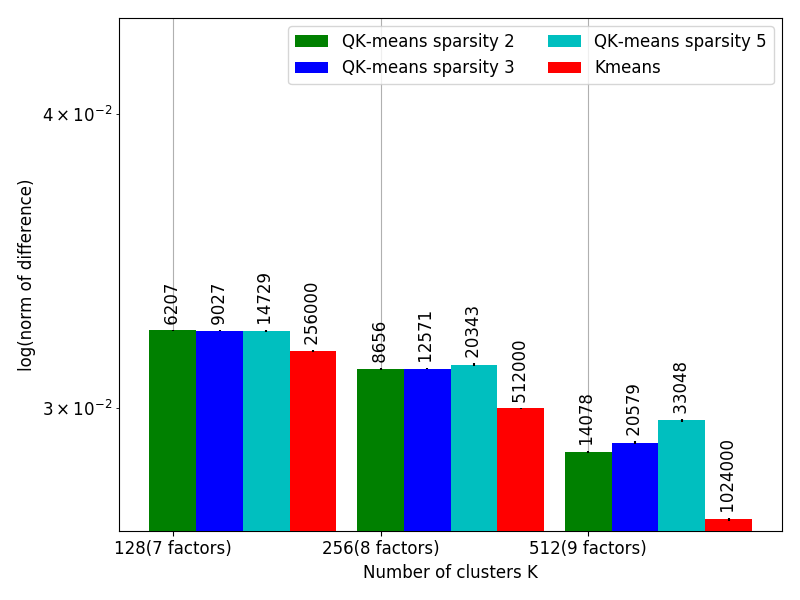
\includegraphics[width=\textwidth]{blobs_nystrom_error.png}
\caption{\texttt{Blobs}: Nyström reconstruction error.}
\label{fig:blobs:nystrom_error}
\end{subfigure}
\begin{subfigure}[b]{.49\textwidth}
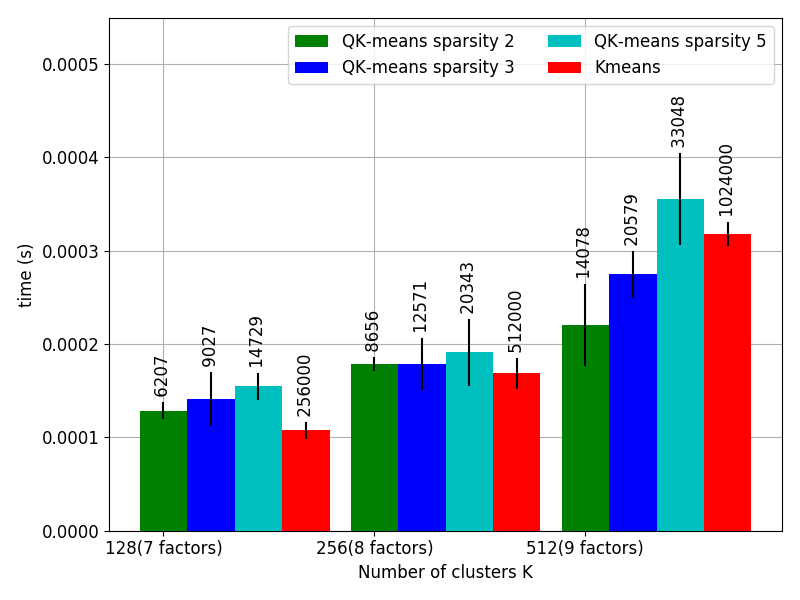
\includegraphics[width=\textwidth]{blobs_nystrom_inference_time.png}
\caption{\texttt{Blobs}: Nyström inference time.}
\label{fig:blobs:nystrom_time}
\end{subfigure}
\begin{subfigure}[b]{.49\textwidth}
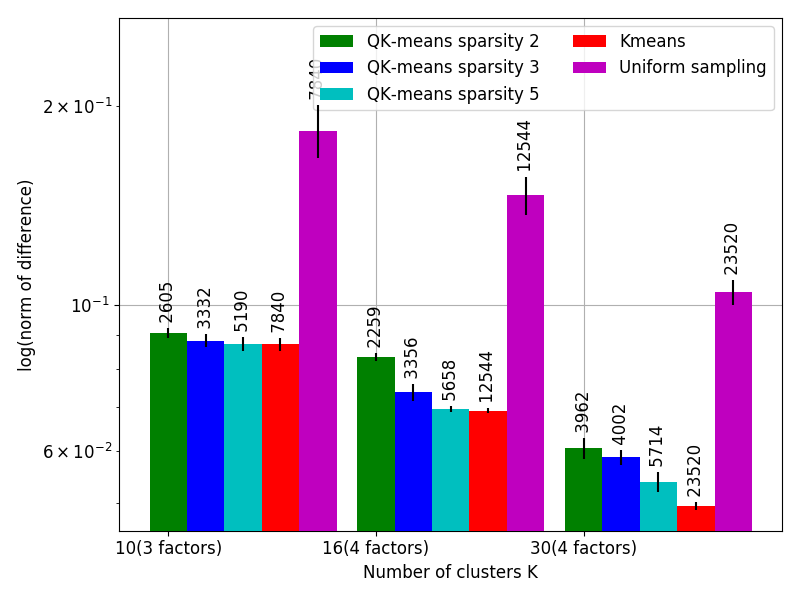
\includegraphics[width=\textwidth]{mnist_nystrom_error.png}
\caption{\texttt{MNIST}: Nyström reconstruction error.}
\label{fig:mnist:nystrom_error}
\end{subfigure}
\begin{subfigure}[b]{.49\textwidth}
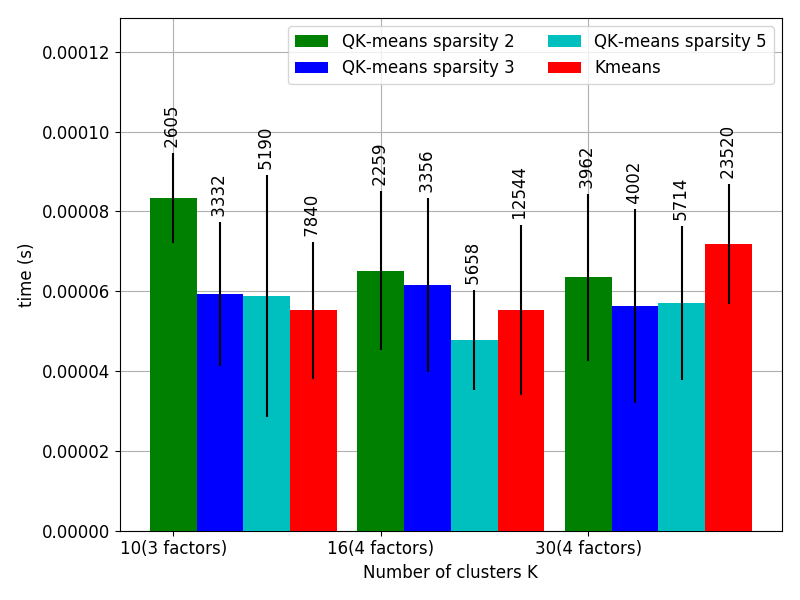
\includegraphics[width=\textwidth]{mnist_nystrom_inference_time.png}
\caption{\texttt{MNIST}: Nyström inference time.}
\label{fig:mnist:nystrom_time}
\end{subfigure}
\begin{subfigure}[b]{.49\textwidth}
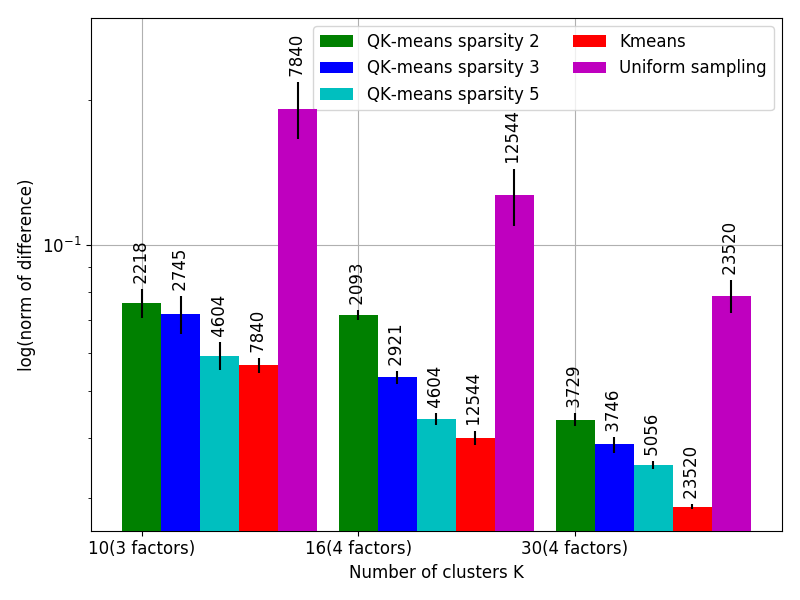
\includegraphics[width=\textwidth]{fashmnist_nystrom_error.png}
\caption{\texttt{Fashion-MNIST}: Nyström reconstruction error.}
\label{fig:fashmnist:nystrom_error}
\end{subfigure}
\begin{subfigure}[b]{.49\textwidth}
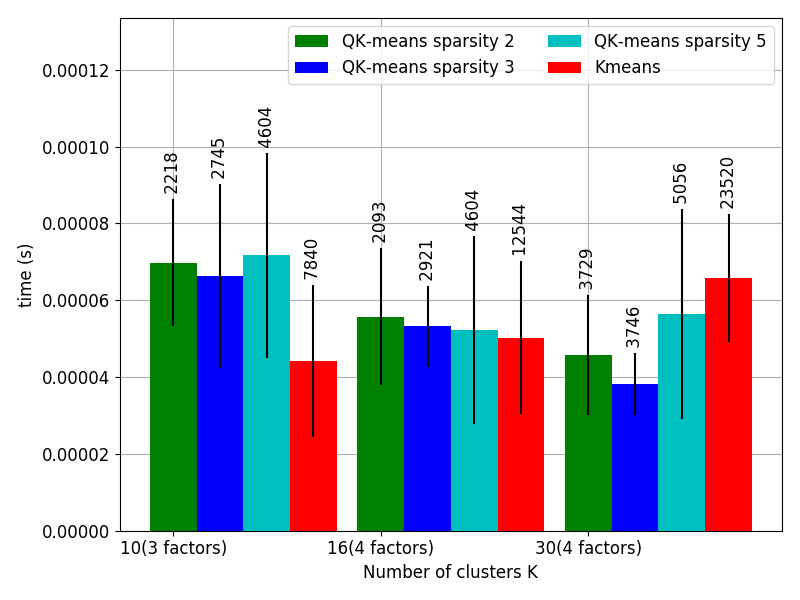
\includegraphics[width=\textwidth]{fashmnist_nystrom_inference_time.png}
\caption{\texttt{Fashion-MNIST}: Nyström inference time.}
\label{fig:fashmnist:nystrom_time}
\end{subfigure}
\caption{Nystr\"om approximation results: accuracy (left) and running times (right). The uniform sampling based Nyström approximation running times are not displayed because they are the same as for the Nyström approximation based on \kmeans centroids. Every experiment results are averaged over 5 runs. The vertical black lines are the standard deviation w.r.t. the runs.}
\label{fig:nystrom}
\end{figure*}

%{RBF networks}

%Besoin d'éclaircir les liens avec RBF networks

%\subsection{nearest-neighbours}

%Besoin d'éclaircir les liens avec nearest neighbours
